\documentclass{article}
\usepackage{listings}
\usepackage{graphicx}
\usepackage{amsmath}
\usepackage{minted}
\usepackage[margin=1in]{geometry}
\usepackage{xcolor}


\definecolor{codegreen}{rgb}{0,0.6,0}
\definecolor{codegray}{rgb}{0.5,0.5,0.5}
\definecolor{codepurple}{rgb}{0.58,0,0.82}
\definecolor{backcolour}{rgb}{0.95,0.95,0.99}
\lstdefinestyle{mystyle}{
    backgroundcolor=\color{backcolour},   
    commentstyle=\color{codegreen},
    keywordstyle=\color{magenta},
    numberstyle=\tiny\color{codegray},
    stringstyle=\color{codepurple},
    basicstyle=\ttfamily\footnotesize,
    breakatwhitespace=false,         
    breaklines=true,                 
    captionpos=b,                    
    keepspaces=true,                 
    numbers=left,                    
    numbersep=5pt,                  
    showspaces=false,                
    showstringspaces=false,
    showtabs=false,                  
    tabsize=2
}
\lstset{style=mystyle}
\begin{document}

\title{ELCT 432 Computer Assignment \#5}
\author{Jacob C. Vaught}
\date{\today}

\maketitle

\section*{Task 1: Transmitter}

\subsection*{Introduction}
The objective of this task is to construct an FM transmitter using MATLAB. The transmitter is designed to transmit the signal $cos(2\pi f_m t)$ over a duration of 20 ms where $f_m = 20$ KHz.

\subsubsection*{Specifications}
\begin{itemize}
    \item Modulation index: 5
    \item Carrier frequency, $f_c$: 913 MHz
    \item Sampling frequency, $f_s$: 2 Msps
\end{itemize}

\subsection*{Analysis}

\subsubsection*{Baseband Signal}
The baseband signal is:
\[ x(t) = cos(2\pi f_m t) \]
For $f_m = 20$ KHz.
\[ x(t) = cos(40000\pi t) \]

\subsubsection*{Bandpass Signal for FM}
Given the carrier frequency \( f_c = 913 \) MHz and the baseband signal \( x(t) = \cos(2\pi f_m t) \), the FM modulated signal, considering a constant amplitude \( A \), is:
\[ x_{BP}(t) = A \cos\left(2\pi f_c t + m \frac{\sin(2\pi f_m t)}{2\pi f_m}\right) \]
\[ x_{BP}(t) = A \cos\left(2\pi 913e6 t + 5 \frac{\sin(40000\pi t)}{40000\pi}\right) \]

\subsubsection*{Bandwidth using Carson's Rule}
Given the modulation index $m = 5$ and $f_m = 2$ KHz, the frequency deviation $f_\Delta$ is:
\[ f_\Delta = m \times f_m \]
\[ f_\Delta = 5 \times 20\, \text{KHz} = 100\, \text{KHz} \]
Using Carson’s rule, the bandwidth, $B$, is:
\[ B = 2(f_m + f_\Delta) \]
\[ B = 2(20\, \text{KHz} + 100\, \text{KHz}) = 240\, \text{KHz} \]

\subsubsection*{Spectrum of the Bandpass Signal}
For a theoretical analysis, the spectrum of the bandpass signal can be plotted. \begin{center}
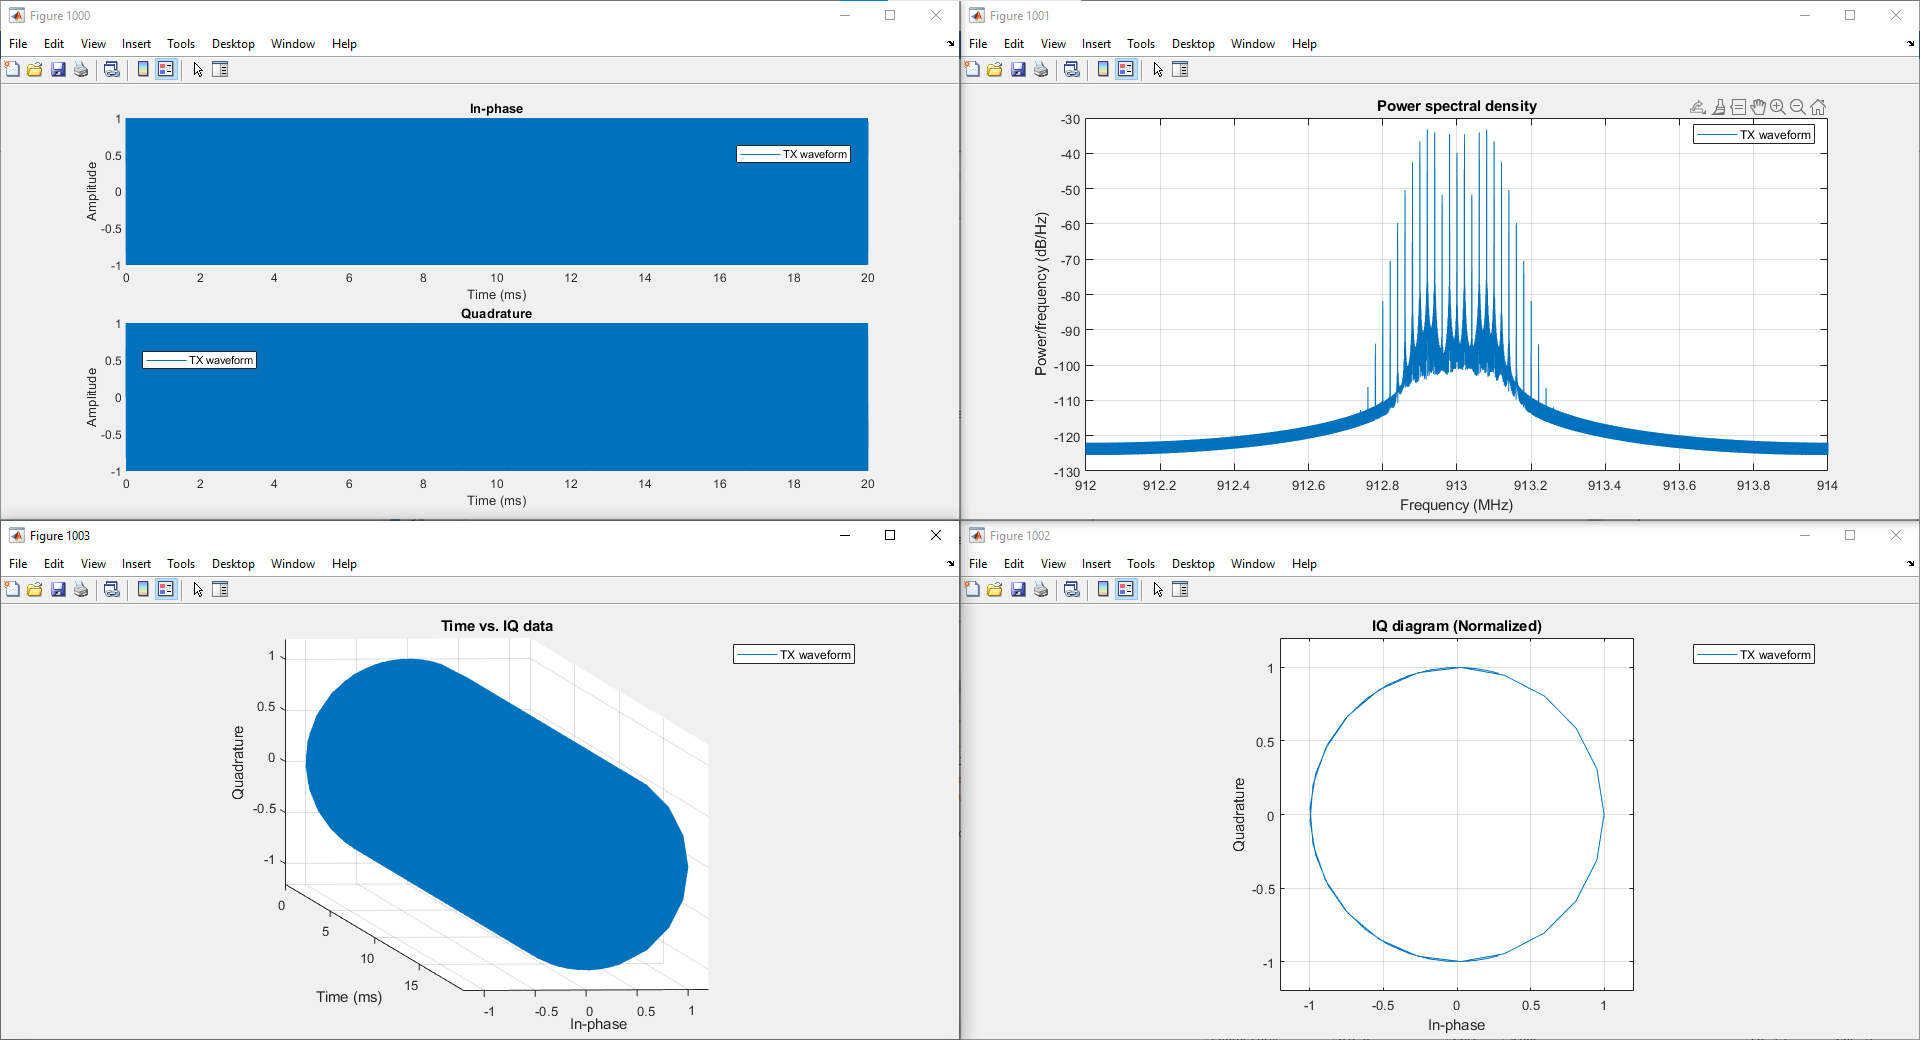
\includegraphics[width=1\textwidth]{T1_bandpass_ML.png}
\end{center}

\subsection*{MATLAB Code}
\lstinputlisting[language=Octave]{transmit.m}

\subsection*{Code Explanation}

\subsubsection*{Establishing Connection to PlutoSDR}
The script starts by clearing variables, closing open figures, and clearing the command window with `clear all`, `close all`, and `clc` commands respectively. 

Next, the sampling frequency `fsample` is set to 2e6 (2 Msps) and the carrier frequency `fc` to 913e6 (913 MHz). The script then sets up a connection to the PlutoSDR transmitter with the given IP address and other parameters like gain, center frequency, and baseband sample rate.

\subsubsection*{Generating IQ Data for FM Modulated Signal}
The number of samples, `Nsamples`, is determined based on the desired signal length and the sampling frequency. A time vector `timeSamples` is then generated for the specified number of samples.

The message frequency `fm` is set to 20e3 (20 kHz). An anonymous function `sb` is defined to produce the IQ data for the FM modulated signal. The IQ data, `IQdataTX`, is then generated using this function for the given time samples.

\subsubsection*{Waveform Normalization}
Normalization is essential for software-defined radio operations to ensure that the maximum absolute value of the transmitted signal does not exceed the acceptable range. The script checks the maximum value of the generated IQ data, and if it's not zero, it normalizes the data to ensure its maximum absolute value is less than or equal to 1.

\subsubsection*{Analyzing the Generated Waveform}
Various visualization options are set to true, allowing the user to view the generated waveform in the time domain, its power spectral density, its IQ diagram, and a 3D representation of the time domain signal. The function `analyzeIQdata` is then called with the generated IQ data and visualization options to produce the desired plots.


\subsection*{Results Validation with GNURadio}
Upon receiving the signal with GNURadio, the signal spectrum and other properties were analyzed. 
\begin{center}
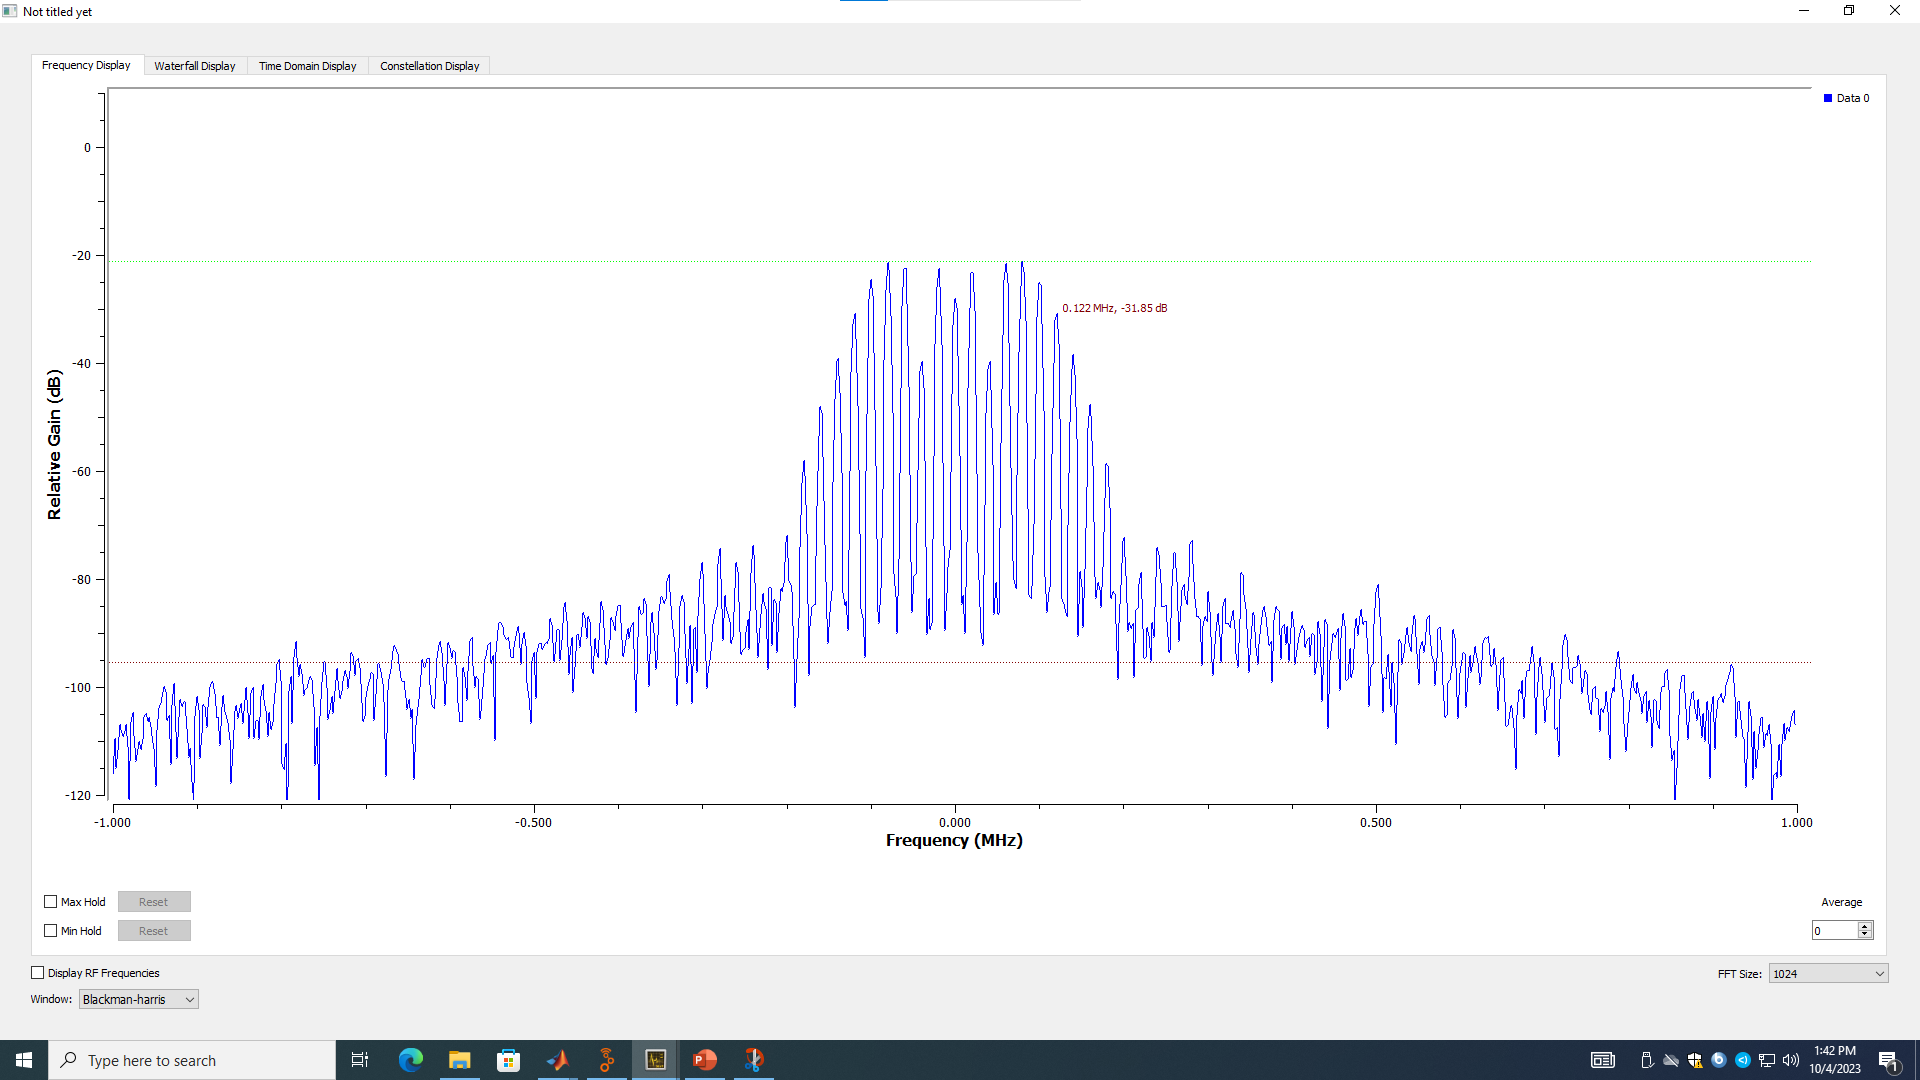
\includegraphics[width=1\textwidth]{T1_GNU_up.png}
\end{center}
\begin{center}
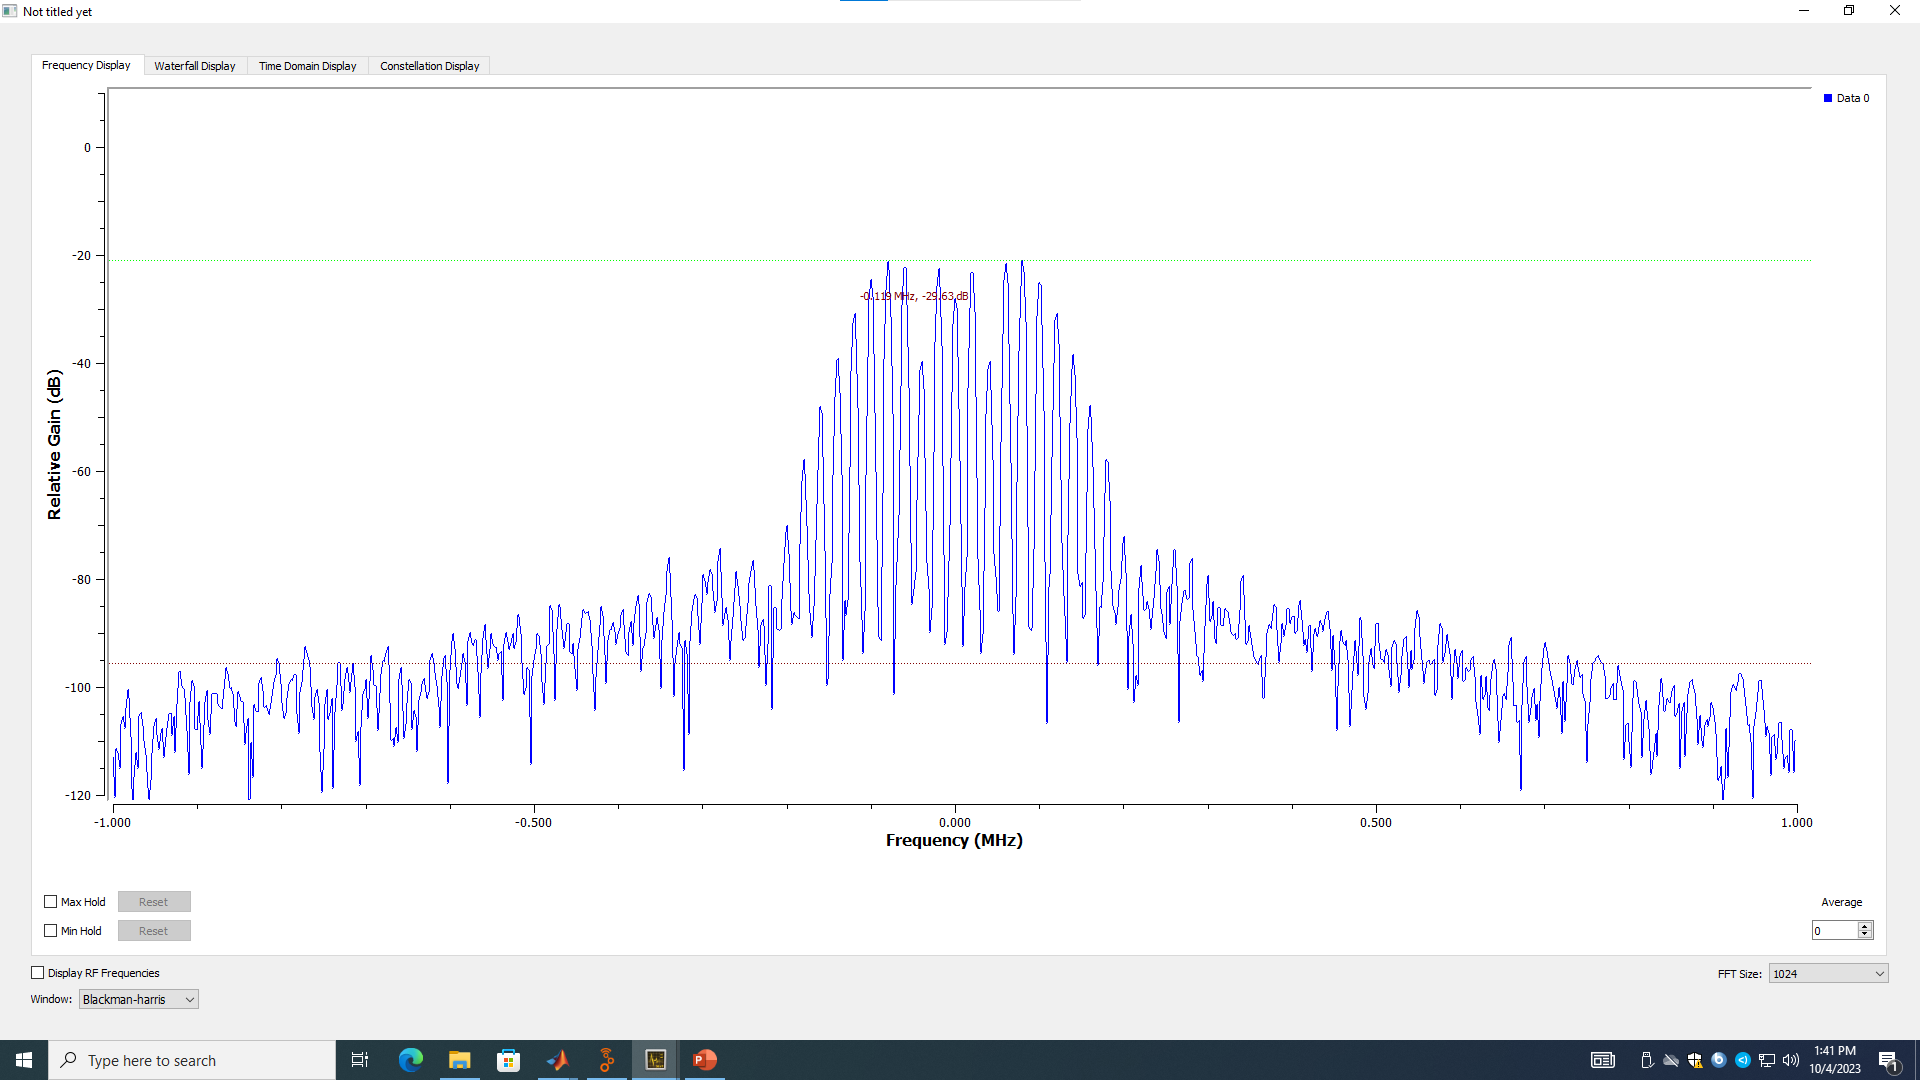
\includegraphics[width=1\textwidth]{T1_GNU_down.png}
\end{center}
The results from GNURadio matched the MATLAB results, and the bandwidth matched what was calculated, at 240 kHz(note -0.119 and 0.122 MHz shows that eh bandwidth is close to 240 kHz).
The Bessel function of the radio waves is also visible.

\newpage
\section*{Task 2: Receiver}

The task involves creating an FM Radio in MATLAB with the following specifications: 
\begin{itemize}
    \item Center frequency, \(f_c\): 93.5 MHz
    \item Sampling frequency, \(f_s\): 2 Msps
    \item SDR gain: 50 dB
\end{itemize}

\subsection*{MATLAB Implementation for Capturing IQ Data}
The provided MATLAB script first sets up a connection to the PlutoSDR receiver. This is followed by the capture of IQ data for a duration of 5 seconds and the subsequent analysis of the received waveform. This code recives and analyzes the 93.5 MHz signal.

\lstset{language=Octave}
\begin{lstlisting}
fc = 93.5e6;
fsample = 2e6;
rxPluto = sdrrx('Pluto', 'RadioID','ip:192.168.2.4', 'GainSource','Manual',...
'Gain', 50,'CenterFrequency',fc, 'OutputDataType', 'double','EnableBurstMode', false, ...
'SamplesPerFrame', 10000000,'BasebandSampleRate',fsample);
rxPluto.ShowAdvancedProperties = true;
IQdataRX = rxPluto();
options.showTimeDomainSignal = 1;
options.showPowerSpectralDensity = 1;
options.showIQDiagram = 1;
options.showTimeDomainSignal3D = 0;
options.fsample = fsample;
options.fcarrier = fc;
options.figureName = 'RX waveform';
options.figurePositionsOption = 1; 
analyzeIQdata(IQdataRX, options)
\end{lstlisting}

\subsection*{Analysis of the Received IQ Data}
After capturing the IQ data, we can see that the FM signal exists in the spectrum.

\begin{center}
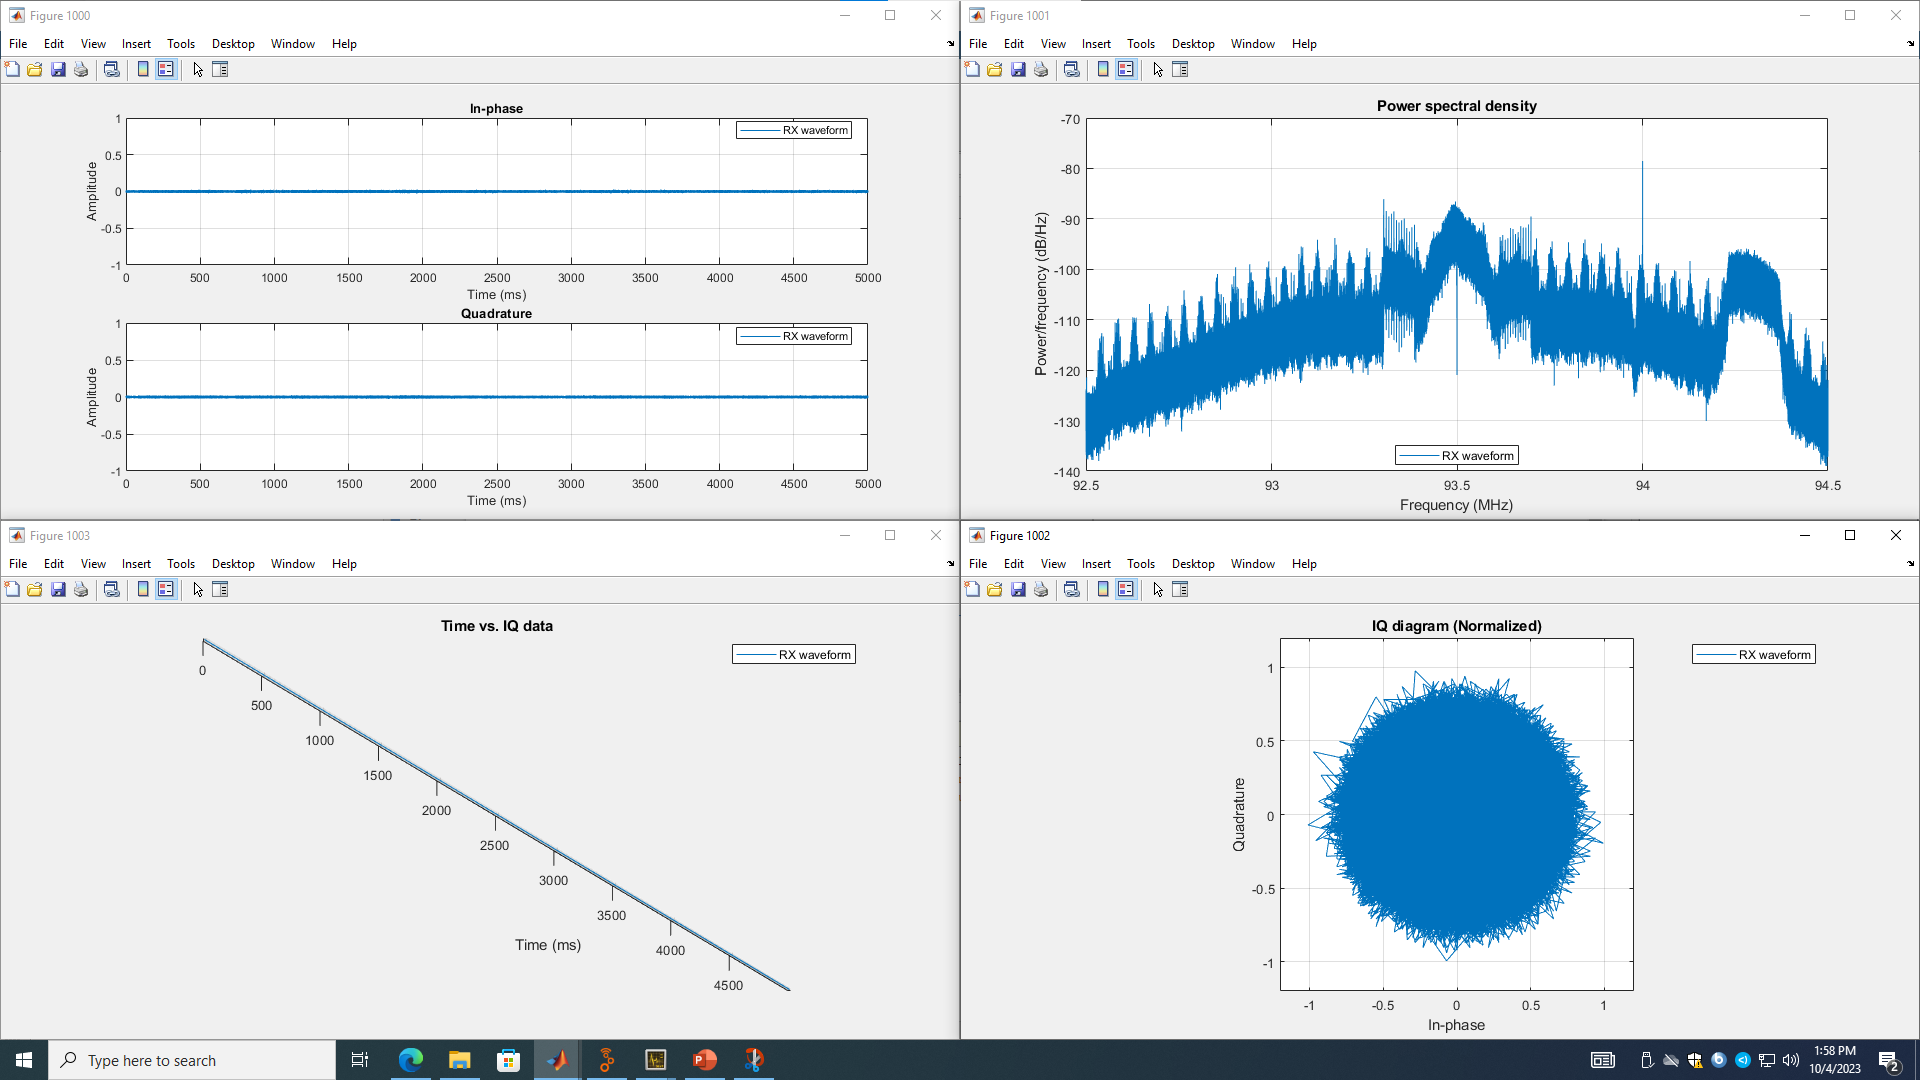
\includegraphics[width=1\textwidth]{T2_signal_ML.png}
\end{center}

\subsection*{Demodulating the FM Signal}

Frequency Modulation (FM) demodulation can be accomplished in several ways, but a common method in digital signal processing is to differentiate the phase of the received signal, which is effectively the instantaneous frequency. The provided MATLAB code snippet accomplishes this in a few steps:

\begin{enumerate}
    \item \textbf{Phase Extraction and Unwrapping:} The `angle' function extracts the phase of the complex IQ data `IQdataRXa'. Due to the nature of the arctangent function used in phase extraction, the phase will wrap around when it exceeds its range. The `unwrap' function is employed to remove such discontinuities from the phase data.
    
    \begin{lstlisting}
    unwrap(angle(IQdataRXa))
    \end{lstlisting}
    
    \item \textbf{Differentiation:} Differentiating the unwrapped phase data yields the instantaneous frequency deviation from the carrier frequency. The `diff' function computes the difference between consecutive elements of the unwrapped phase data.

    \begin{lstlisting}
    x=diff(unwrap(angle(IQdataRXa)));
    \end{lstlisting}
    
    \item \textbf{Normalization:} The differentiated data is then normalized by dividing by \(2\pi \times 75e3\) (where 75 kHz is a typical frequency deviation for FM broadcast) to convert the frequency deviation to a voltage level suitable for audio.

    \begin{lstlisting}
    y=x/(2*pi*75e3);
    \end{lstlisting}
    
    \item \textbf{Accounting for Data Length:} Since differentiation reduces the length of the data by one, the first element of `y' is replicated to make its length consistent with the original data.

    \begin{lstlisting}
    y=[y(1);y];
    \end{lstlisting}
    
    \item \textbf{Downsampling:} To convert the sampled data to a standard audio rate (200 ksps in this case), the signal is downsampled by a factor of 10.

    \begin{lstlisting}
    y_r=downsample(y, 10);
    \end{lstlisting}
    
    \item \textbf{Playing Audio:} Finally, the `soundsc' function plays the demodulated audio signal at the desired sampling rate of 200 ksps.

    \begin{lstlisting}
    soundsc(y_r, 200e3);
    \end{lstlisting}
\end{enumerate}

\newpage
\subsection*{Audio Signal Visualization}
This first image is the filtered version of the audio, after filtering the FM spectrum.
\begin{center}
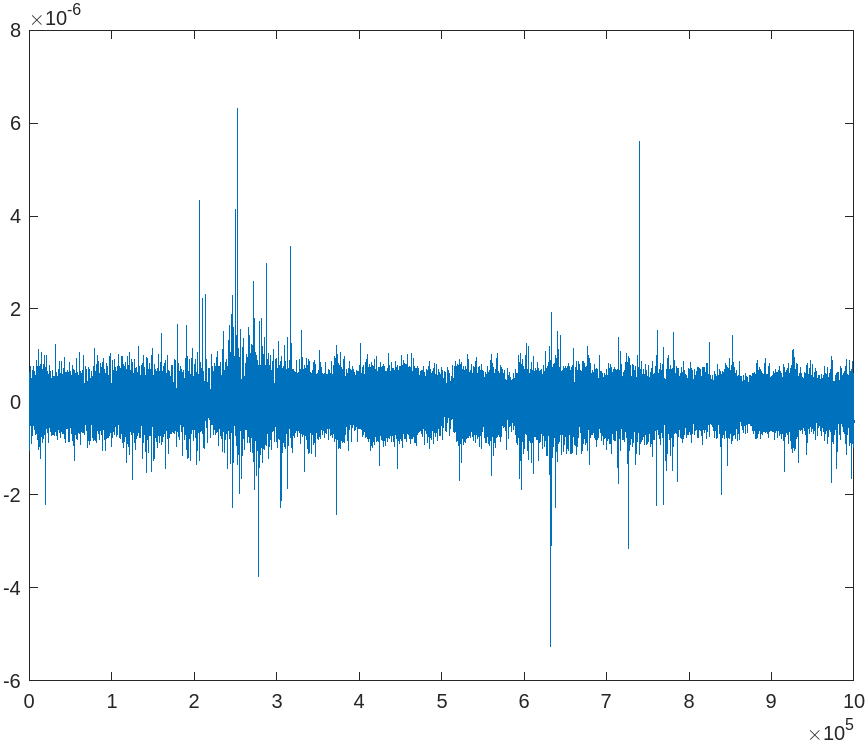
\includegraphics[width=0.7\textwidth]{T2_audio_filter.png}
\end{center}

This is what the sound looks like before filtering. There is a lot of noise affecting the results. 
\begin{center}
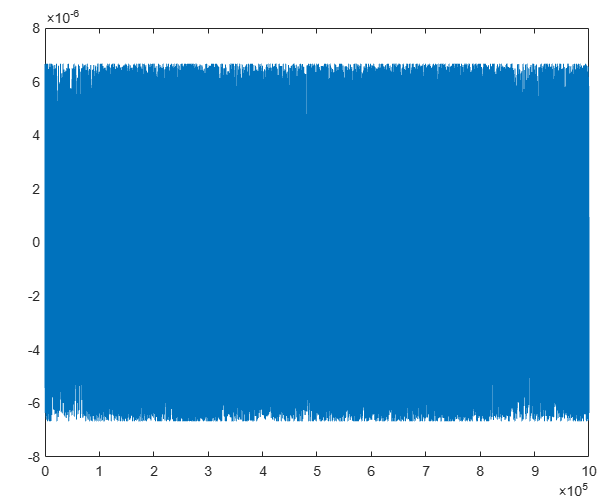
\includegraphics[width=0.7\textwidth]{T2_audio_no_filter.png}
\end{center}
\newpage
\subsection*{Improving Sound Quality}
The sound quality can be improved by employing a low pass filter to eliminate unnecessary data from other frequencies. The proposed method involves filtering out components that do not belong to the desired FM band.
\newline
\textbf{Filter details:}
The MATLAB code snippet for filter design is provided below:

\lstset{language=Octave}
\begin{lstlisting}
% The following code was used to design the filter coefficients:
% % Equiripple Lowpass filter designed using the FIRPM function.
%
% % All frequency values are in Hz.
% Fs = 2000000;  % Sampling Frequency
%
% Fpass = 100000;          % Passband Frequency
% Fstop = 120000;          % Stopband Frequency
% Dpass = 0.057501127785;  % Passband Ripple
% Dstop = 0.0001;          % Stopband Attenuation
% dens  = 20;              % Density Factor
\end{lstlisting}

\subsection*{Complete MATLAB Code for the Task}
The entire code for the task, including IQ data capture, analysis, FM demodulation, and audio signal visualization, is presented below.

\lstinputlisting[language=Octave]{receiver.m}
\end{document}
